% !TEX root = ../toptesi-scudo-example.tex
% !TEX encoding = UTF-8 Unicode
%***********************************************************************
%***********************************Fourth Chapter
%***********************************************************************

\chapter{Simulator}
\label{chap:5_simulator}
	\graphicspath{{Chapter5/}}


\begin{itemize}
	\item introduzione, dove spiego la necessita di un simulatore
	\item struttura del simulatore + algoritmo
	\item chartging station palcement + grafiici (avg time, num parking)
	\item charging policies
\end{itemize}

\section{Abstract}
in this chapter I describe mainly the simulator ...

\section{Introduction}
The aim of this work is to find a methodology to convert combustion engine FFCS into electric one using real data. In order to do that,  I developed an event-driven simulator able to replicate the users' FFCS mobility patterns created from the data collected with the tools described in chapters \ref{chap:2_dataset} and \ref{chap:4_cs_comparison}. 

In order to give a main idea, the simulator takes as input a real trace composed by a ordered set of rentals, an operative area composed by adjacent squares zones of 0.025 $km_2$, the set of charging station and their placement, a car model and a fleet size. By consuming the trace, the simulator computes trip by trip the amount of energy needed to travel the proper distance and moves the designed car from the starting point to the chosen destination.

During the simulations, the software computes several metrics in order to measure to proper size the charging infrastructure and how it is refleceted as user discomfort, i.e. in terms of number of plugging operation.

Those metrics are heavily influenced by the some environmental parameters like the number and the distribution of charging station. For this reason I proposed three placement strategies related to users' driving patterns. 

Moreover, an electric vehicle fleet needs a proper return policy to manage the battery state of charge. Indeed, the long charging time implies a smart car release, especially in zones having a charging station. The simulator takes in account this aspect too and compares different car return strategy.

This chapter is organized as follow: section \ref{sec:5_2_modelling} describes the the algorithm behind the simulator, section \ref{sec:5_3_mh_placement} illustrates the charging stations placement, section \ref{sec:5_4_return_policy} explains how I modelled the provider return policed that customers have to follow, section \ref{sec:5_5_kpi_scenario} explains the metrics taken in account and measured by the simulator and finally \ref{sec:5_6_conclusion} concludes the chapter proposing a work resume.

\section{Electric car sharing simulator}
\label{sec:5_2_modelling}

The goal is to study different design choices for electric car sharing systems. For this, I developed a flexible event-based simulator that allows us to compare different algorithms and tune their parameters while collecting metrics of interest. The simulator consumes a trace composed by a subset of rentals collected in \ref{chap:2_dataset}. In this way, by implementing an electric car consumption, I am able to model an electric FFCS provider that exactly replicate customers' temporal and spatial demand.
% Simulations are based on the actual traces collected from operative FFCS providers in each city. This allows to factor all spatial and temporal characteristics of actual FFCS customers habits.

\subsection{Simulation model}

The simulator replicates the behaviour of a fleet of electric cars, which are moving in the city. Each car is characterized by its location, and the current status of battery charge. The simulator takes as input a pre-recorded trace of rentals characterized by the start and end time, and initial and final geographic coordinates.

In more details, each trip $i \in \mathcal{I}$  is characterized by its start and end time, $t_{s}(i)$ and $t_{e}(i)$, and origin and destination coordinates, $o(i)$ and $d(i)$. For simplicity, I divide the city area into squared zones, of side 500\,m as before. Then, I associate with each position one and only one zone $O(i)=zone(o(i))$ and $D(i)=zone(d(i))$. We assume a charging station $cs$, composed of $k$ poles, can be placed at the center of a given zone $z\in \mathcal{Z}$, so either $cs(z)=1$ if the station is present, or $cs(z)=0$ otherwise. $N=\sum_{z\in \mathcal{Z}}cs(z)$ is the total number of zones equipped with charging stations, with 
$K=N\cdot k$ the total number of poles.


Additionally, it is present a set $\mathcal{A}$ of cars, with its cardinality $\left\vert{\mathcal{A}}\right\vert$ obtained by the trace. Each car $a\in \mathcal{A}$ at time $t$ is characterized by its position $p(a,t)$, its zone $P(a,t)=zone(p(a,t))$, and the residual battery capacity $c(a,t)\in[0,C]$, with $C$ being the maximum nominal capacity.

Generally speaking, the simulator processes each rental event $i$ in temporal order. When a \emph{rental-start} event $i$ is processed at time $t=t_{s}(i)$, the simulator chooses randomly one of the most charged available car in the closest zones to the initial position zone $O(i)$. In formulas, we get a car $\bar{a} \in \mathcal{A}$ such that:
\[
c(\bar{a},t) \geq c(\hat{a},t)\ \forall \hat{a} \in \argmin_{a \in A} {dist(O(i), P(a,t))}.
\]
Basically, the simulator mimics the normal behaviour of FFCS customers that use their smartphone to rent the closest car from their position and are worried about vehicle range~\cite{RangeAnxiety}. Notice that this behaviour is independent from whether the car is at a pole being charged or not.
Then, the simulator schedules the event \emph{rental-end} and it makes the car unrentable. When the rental ends fires, all the statistics about the rented car are updated (like battery consumption and new destination). Obviously, the simulator is able to manage all the events, like battery depletion or unavailable cars nearby the rental starts. 

In output, the simulator produces several statistics about system usage and user-related discomfort metrics related to the electric vehicle plugging procedures. 

\subsection{Modelling of rental event}
%A \emph{rental-end} event is then scheduled using the trace final time $t_{e}(i)$ and desired destination location $d(i)$.

When a \emph{rental-start} event $i$ is processed at time $t=t_{s}(i)$, and the simulator looks for a car in the initial position zone $O(i)$. If one or more cars are present, it selects (one among) the most charged car, i.e, get the car $a\in \mathcal{A}$ such that
\[
P(a,t) = O(i) \, \land \, c(a,t) \geq c(a',t)\ \forall a'\mid P(a',t) = O(i),
\]
independently whether the car is at a pole being charged or not.\footnote{We choose this policy because people are worried about vehicle range~\cite{RangeAnxiety}.}

If any car is available, the simulator selects the closest zone to $O(i)$ containing an available car, mimicking the normal behaviour of FFCS customers that use their smartphone to rent the closest car from their position. If any vehicle is present in the 8 eight neighbouring zones, the rental is marked as {\it infeasible}.
A \emph{rental-end} event is then scheduled using the trace final time $t_{e}(i)$ and location $d(i)$.

When car $a$ rental-end event is processed at time $t_{e}(i)$, the simulator makes as available the car in the real position $p(a,t_{e}(i))$. The arrival zones might correspond to the one present in the \emph{rental-end} event, or it might be necessary to manage a slightly user's re-routing due to vehicle plugging procedures. The policies to decide when and how plug the car are described in section \mc{define sezione}. Once the car is released, the simulator updates the battery State of Charge (SoC) by consuming an amount of energy proportional to the real trip distance:
\begin{eqnarray*}
	c(a,t_{e}(i)) = \nonumber \hspace{0cm}   \max{(c(a,t_{s}(i)) - Energy(p(a,t_{s}(i)), p(a,t_{e}(i))), 0)} 
\end{eqnarray*}

%\[
%c(a,t_{e}(i)) = \max{(c(a,t_{s}(i)) - Energy(p(a,t_{s}(i)), p(a,t_{e}(i))), 0)}
%\]
with $Energy(\cdot)$ that models the energy consumed to go from the car origin $p(a,t_{s}(i))$ to the car destination $p(a,t_{e}(i))$.
In case $c(a,t_{e}(i)) = 0$, the trip $i$ is declared {\it infeasible}. 
The discharged car $a$ still performs further trips, all marked as infeasible, until it reaches a charging station.



\section{Meta-Heuristic Charging Stations Placement}
\label{sec:5_3_mh_placement}
In this sections I explain the ratio behind the charging station placement. Indeed, in the previous section I described the structure and simulation policies, while now I define an important environmental variable that will be deeply studied in chapters \mc{references}. I remind that from the rental booking trace, I extrapolate the service area and I divide it into square zones of 500 m of side length. Then, using the number of parking or the average parking time for each zone, the simulator choose which zones equip with a charging station.

\subsection{Problem formalization}
Given a number of charging station $N$, the first objective is to place them in the city area so to let all rentals feasible, i.e., to find a charging stations placement so that
\[
c(a,t_e(i))>0\ \forall a \in \mathcal{A}, \forall  i \in \mathcal{I}
\]
Since I do not make any assumption on the set of trips $\mathcal{I}$, I cannot know a-priori if a solution exists and provide an analytical general solution. Moreover the number of candidate solutions increases as the binomial coefficient ${\left\vert{\mathcal{Z}}\right\vert}\choose\ N$, making ineffective to numerically compute all possibilities. Instead, I will provide a class of greedy algorithms and analyse the performance in our specific cases of $\mathcal{I}$.
In details, each zone $z\in\mathcal{Z}$ is assigned a likelihood $l_z \geq 0$.
We then solve the problem of finding the subset of $N$ zones that maximizes the total likelihood. In formulas, 
$$\max \sum_{z\in\mathcal{Z}} cs(z)l_z$$

subject to:
$$\sum_{z\in\mathcal{Z}} cs(z) = N$$
$$cs(z)\in \{0,1\},  \forall z \in \mathcal{Z}$$

The above optimization problem can be solved by greedily choosing the top $N$ zones, ordered in decreasing likelihood. We compare the performance of different placement algorithms based on different definition of the likelihood.
\begin{itemize}
	\item{\it Random placement}: $l_z$ is an independent and identical distributed random uniform variable, so that charging stations result placed at random;
	\item{\it Average parking time}: $l_z$ is the average parking duration in $z$ as recorded in the trace;
	\item{\it Total number of parkings}: $l_z$ is the total number of parking events recorded in $z$ in the trace;
%	\item{\it Total parking time}: $l_z$ is the total parking time accumulated in $z$ by all cars recorded in the trace. In each zone, it is the product of the two previous metrics.
\end{itemize}
Those heuristics are driven by the intuition that placing charging stations in those zones where cars are parked for long time (average parking time) or frequently parked (total number of parkings) could improve system performance.


\begin{figure}[th]
	\centering     %%% not \center
	\subfloat[\centering Turin]{{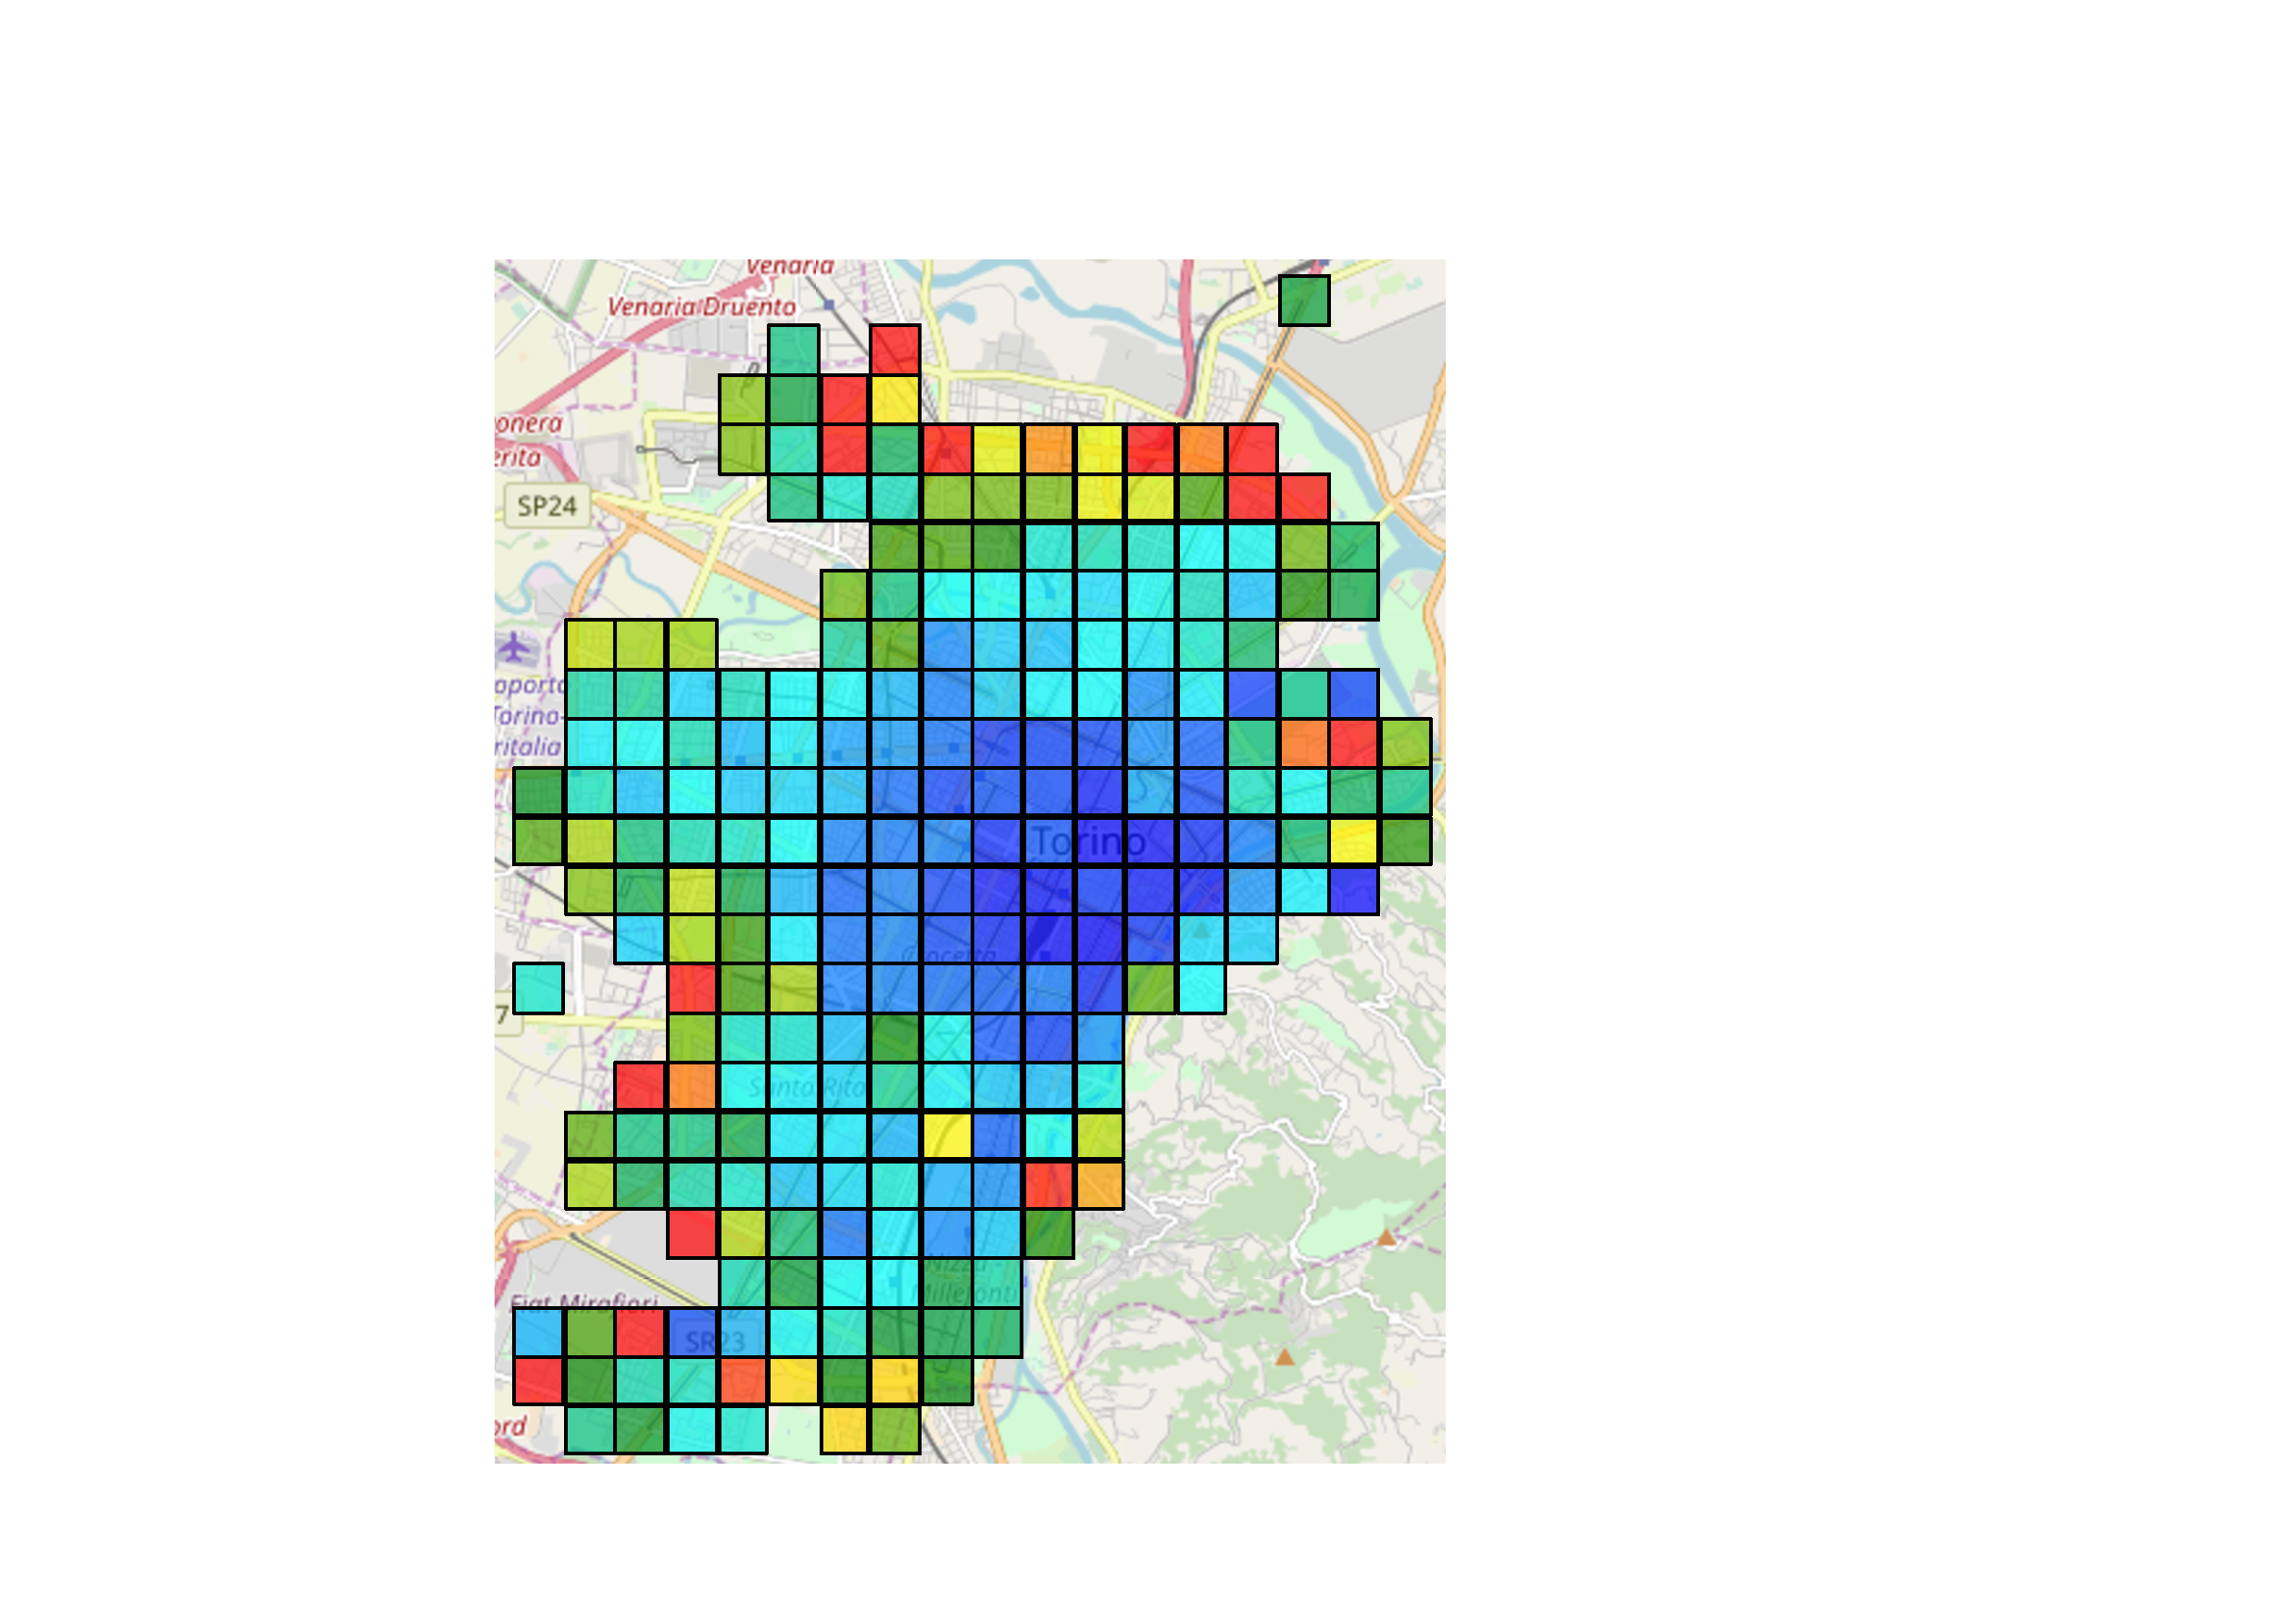
\includegraphics[width=0.22\columnwidth]{figures/Torino_AvgTime.pdf}}\label{fig:5_4_ap_turin}}
	\quad
	\subfloat[\centering Vancouver]{{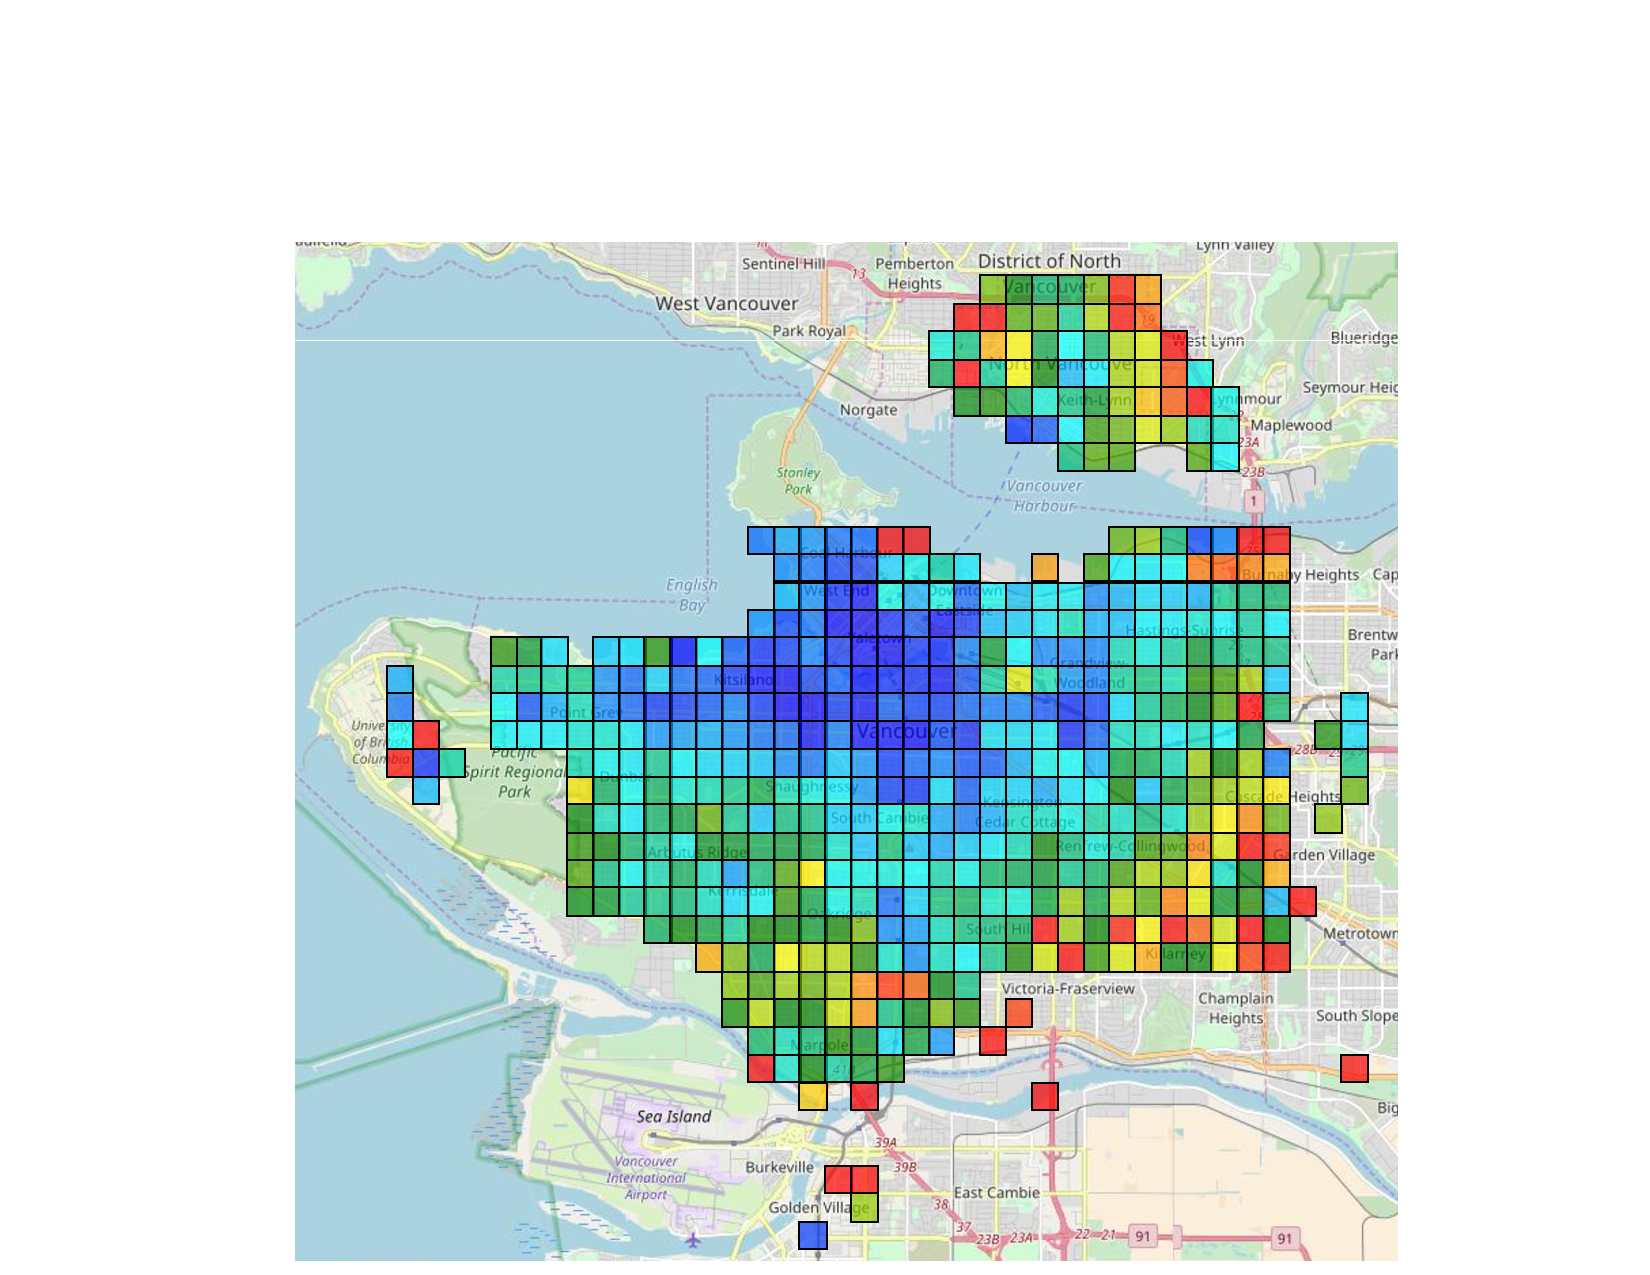
\includegraphics[width=0.30\columnwidth]{figures/VancouverAvgParking.pdf}}\label{fig:5_4_ap_vancouver}}
	\quad
	\subfloat[\centering Berlin]{{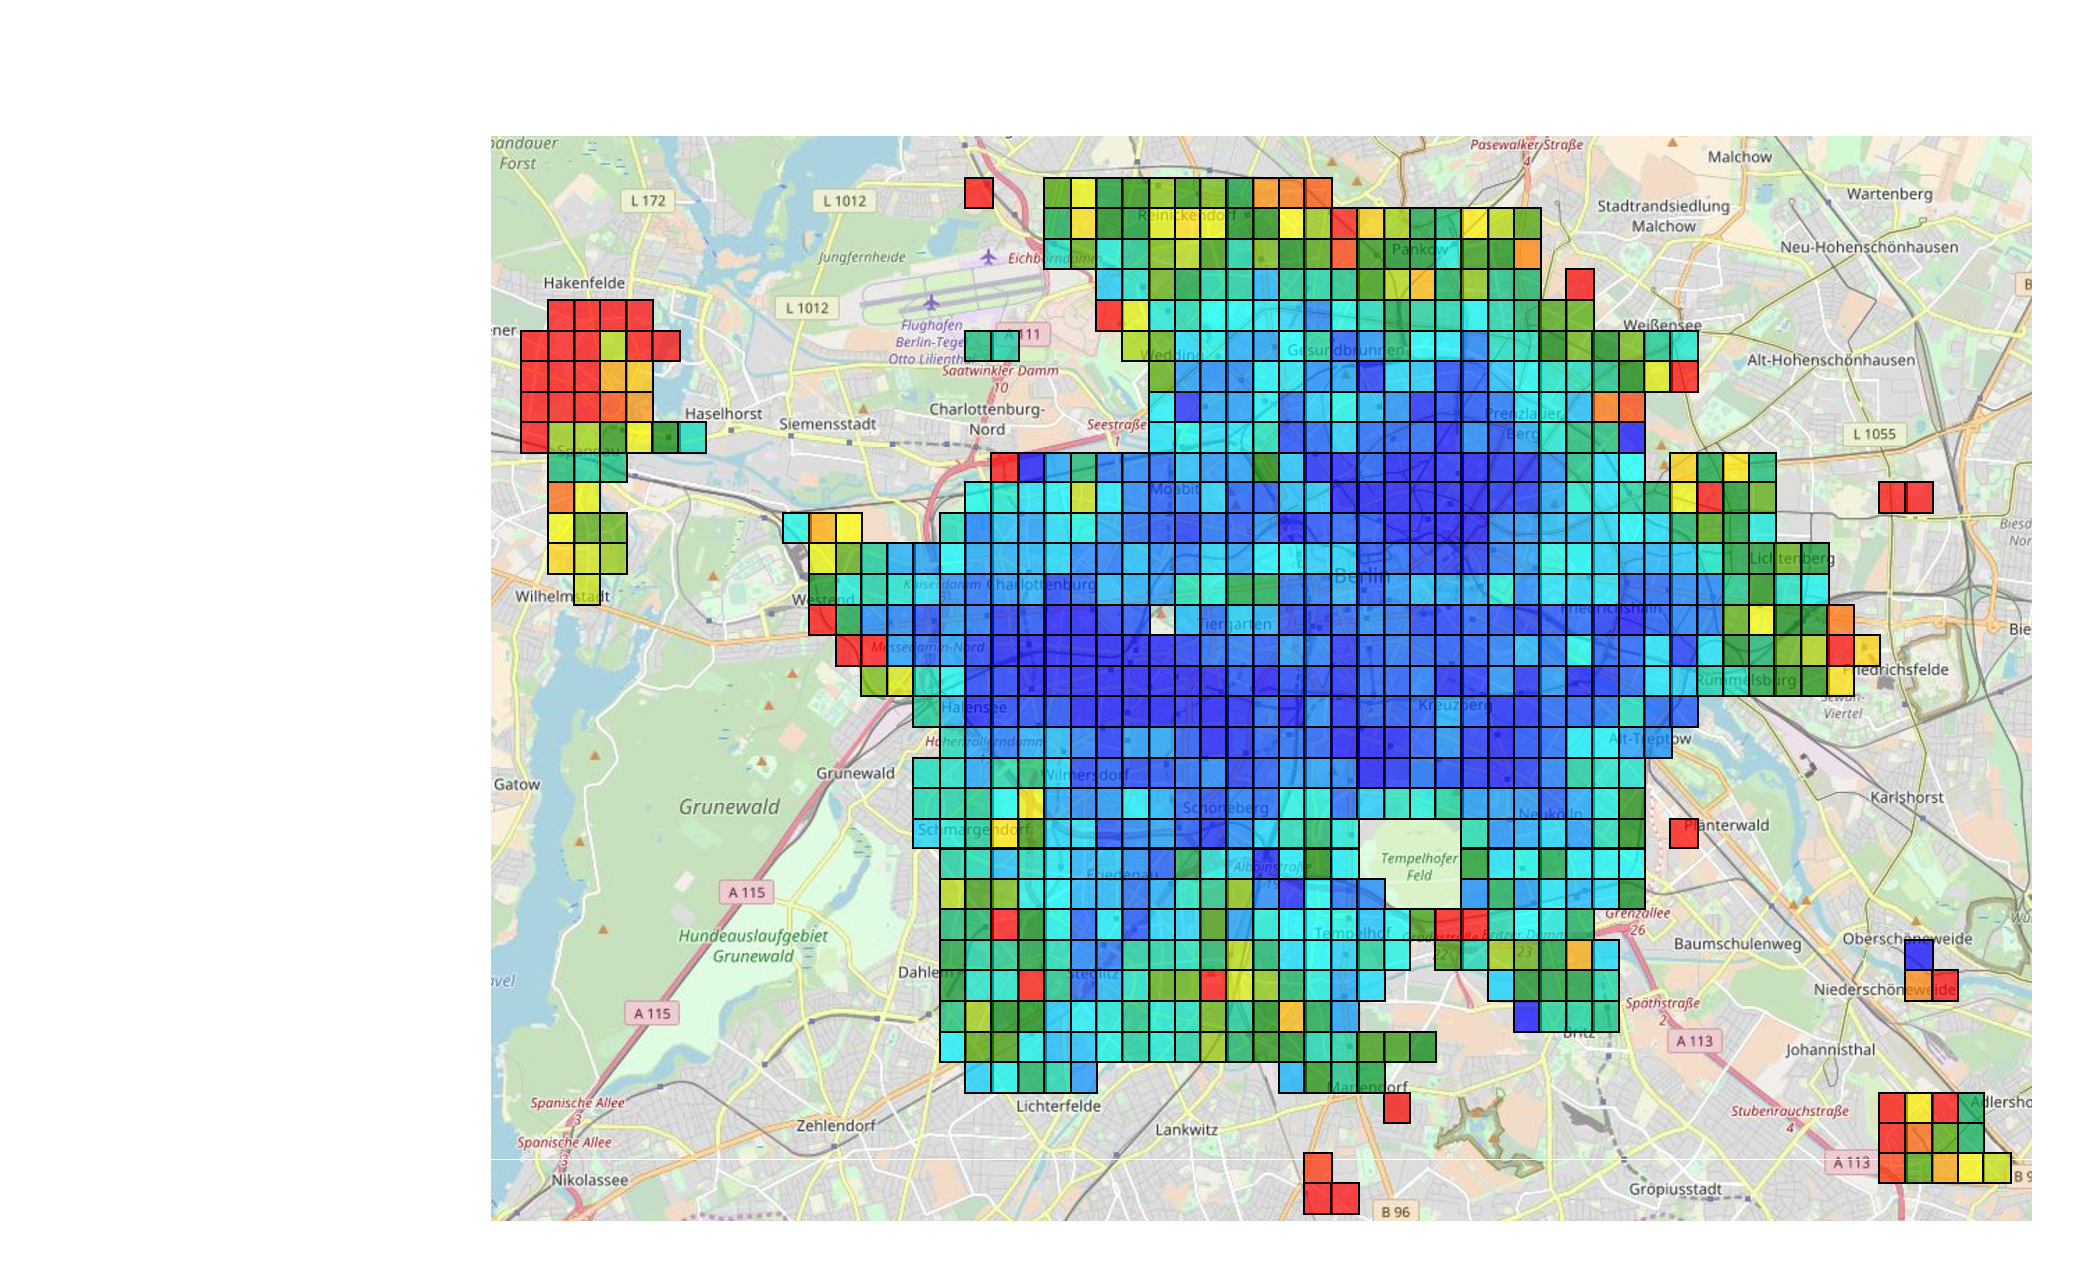
\includegraphics[width=0.4\columnwidth]{figures/BerlinoAvgParking.pdf}}\label{fig:5_4_ap_berlin}}%
	\caption{Distribution of average parking time in Turin, Vancouver and Berlin}
	\label{fig:5_4_heatmap_avgparking}
\end{figure}

I order to show the differences between the likelihoods $l_z$ criteria, figures \ref{fig:5_4_heatmap_avgparking} where $l_z$ is depicted for Turin (\ref{fig:5_4_ap_turin}), Vancouver (\ref{fig:5_4_ap_vancouver}) and Berlin (\ref{fig:5_4_ap_berlin}). The first two cities were deeply characterized in chapters \ref{chap:3_charact} and \ref{chap:4_cs_comparison}, while Berlin, as I will show, presents some interesting spatial distribution. In all the figures, in particular, the more the zone is red, the higher is $l_z$. It means that the \emph{redest} zones will be the first to host a charging station.

In first approach it is possible to se how, in all figures, the heuristic \textit{Average parking time} is mainly spread in city peripheries. It means that the cars spend a lot of times parked far from city centre. This peculiarity can be imputed to commuting patterns: as figure \ref{fig:bookingsweek} points out, two peaks are present in the users' demand. In particular the evening peak catches the back-home commuting which, usually is directed to high-density residential area located in periphery. This, joint with the low business-days night demand, leads to users to leave cars parked in that areas all night long.


\begin{figure}[th]
	\centering     %%% not \center
	\subfloat[\centering Turin]{{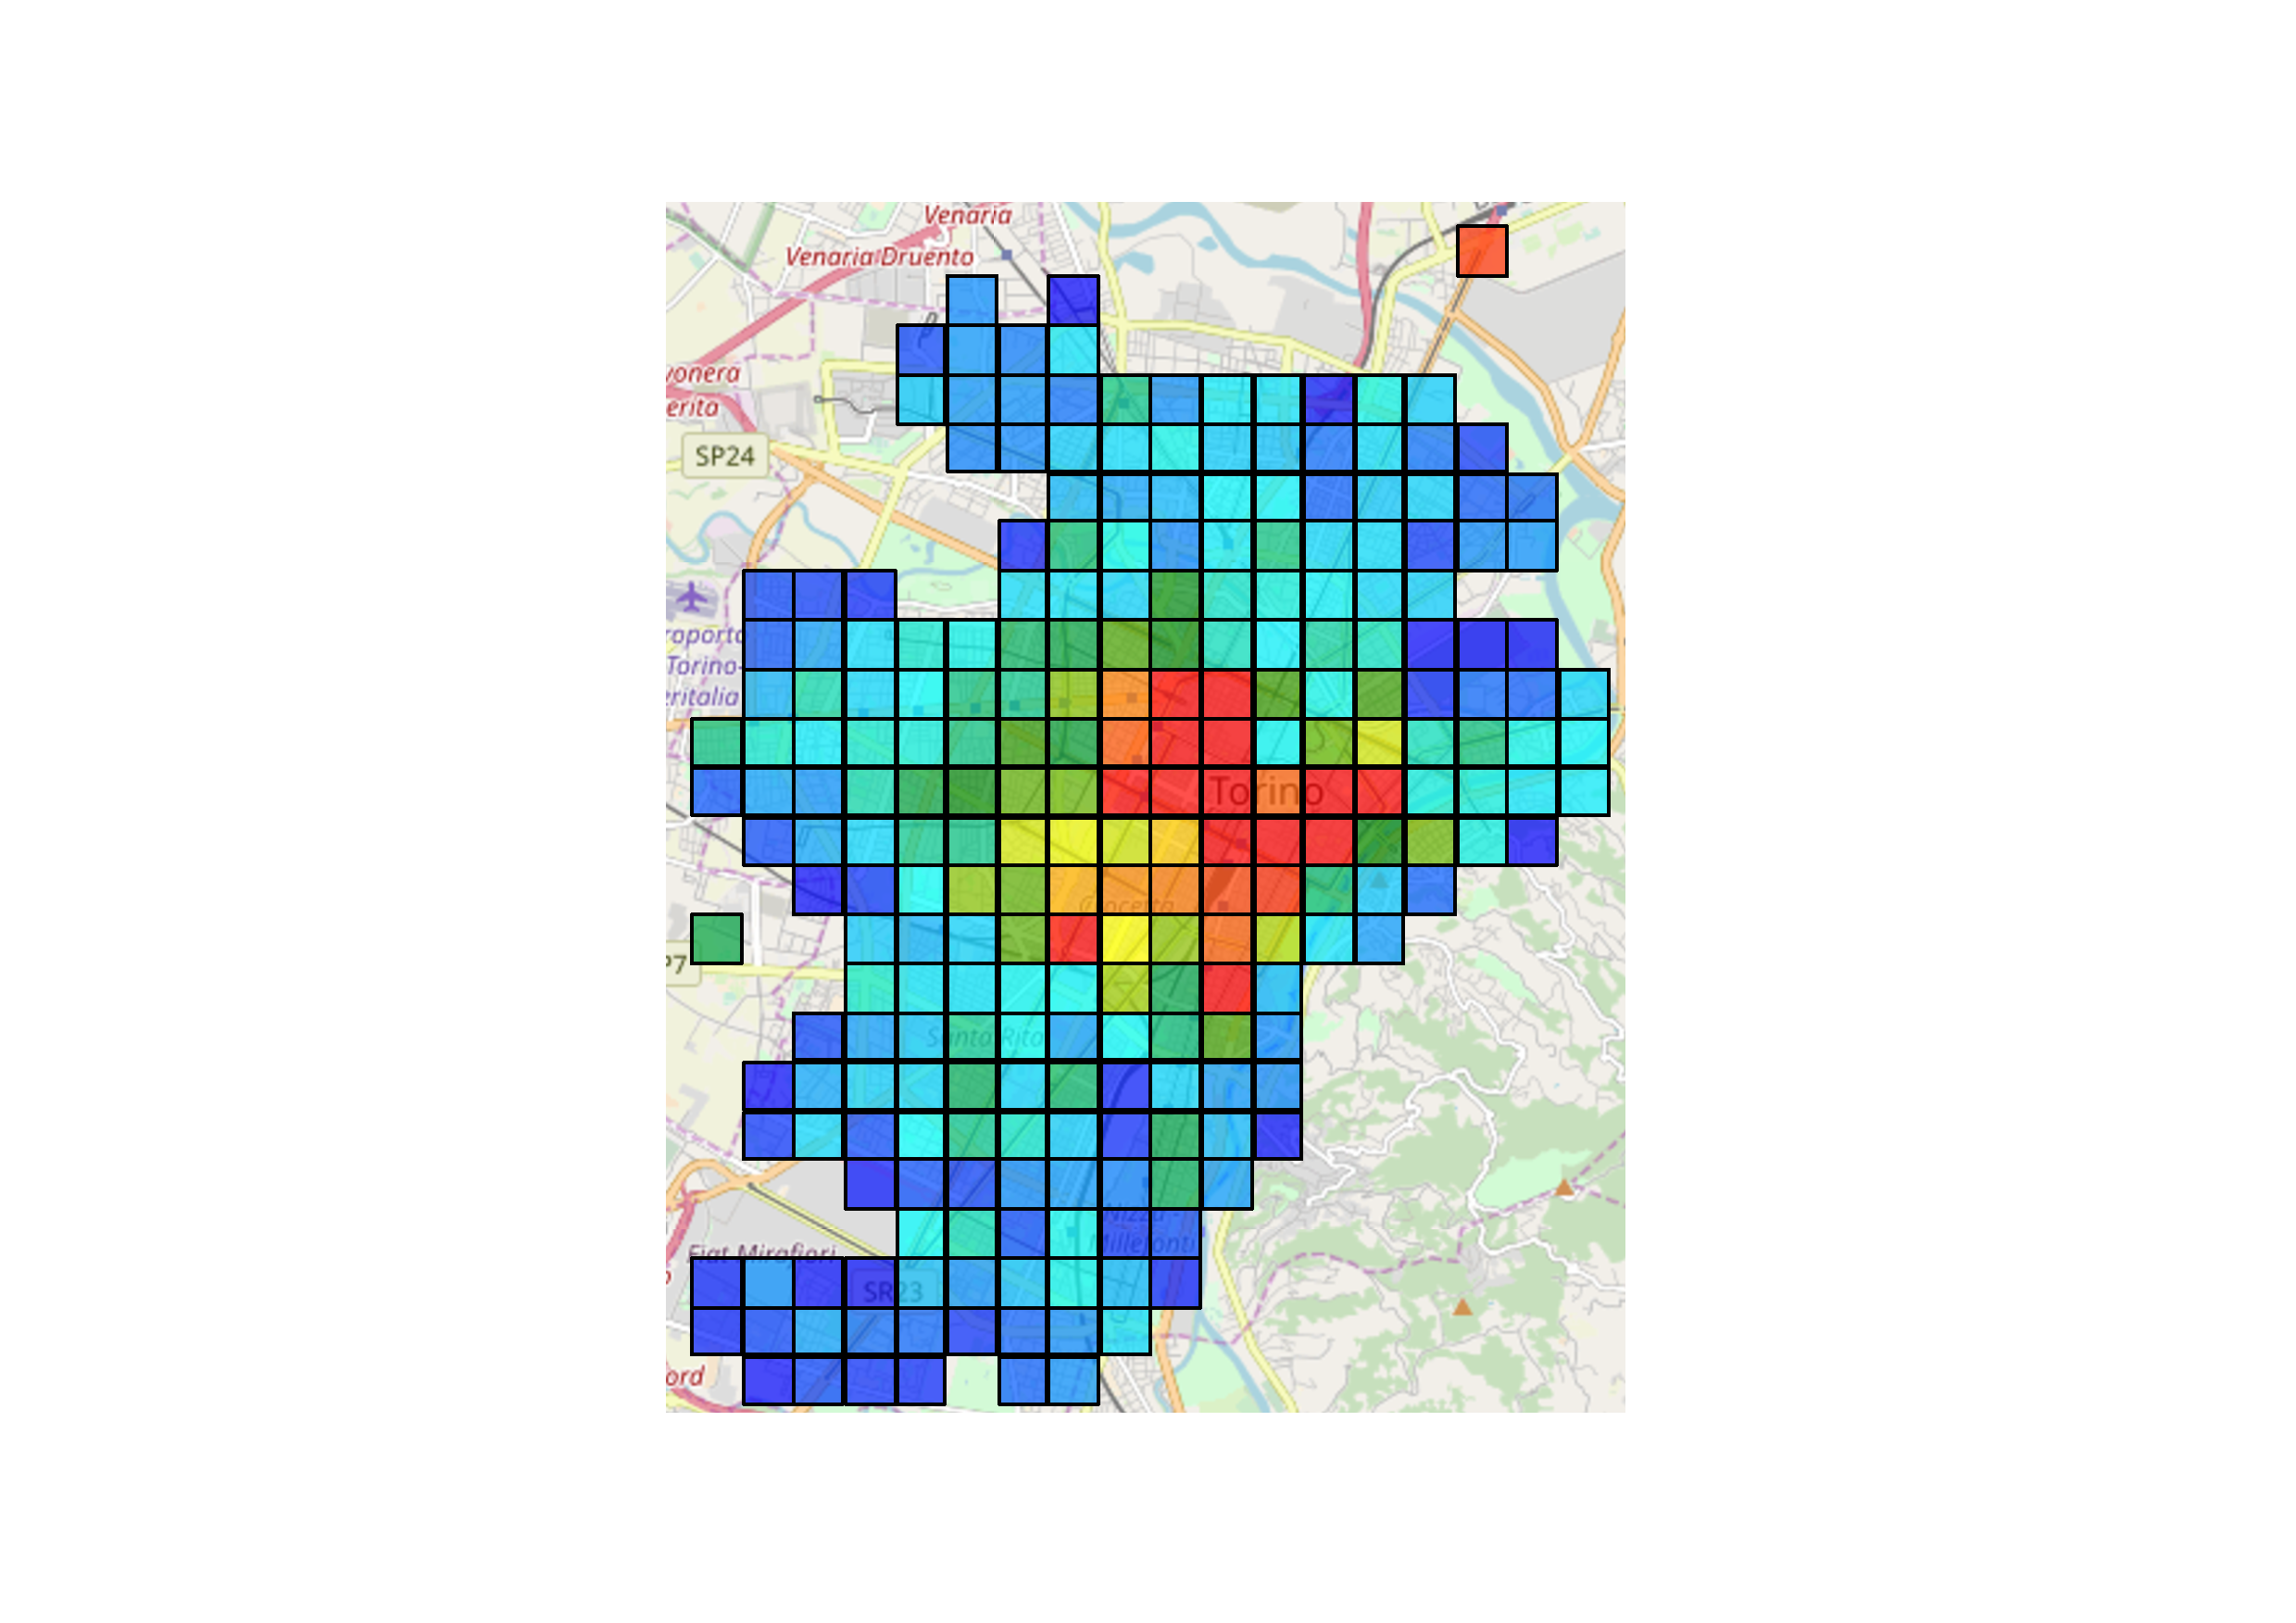
\includegraphics[width=0.22\columnwidth]{figures/Torino_NParkings.pdf}}\label{fig:5_4_np_turin}}
	\quad
	\subfloat[\centering Vancouver]{{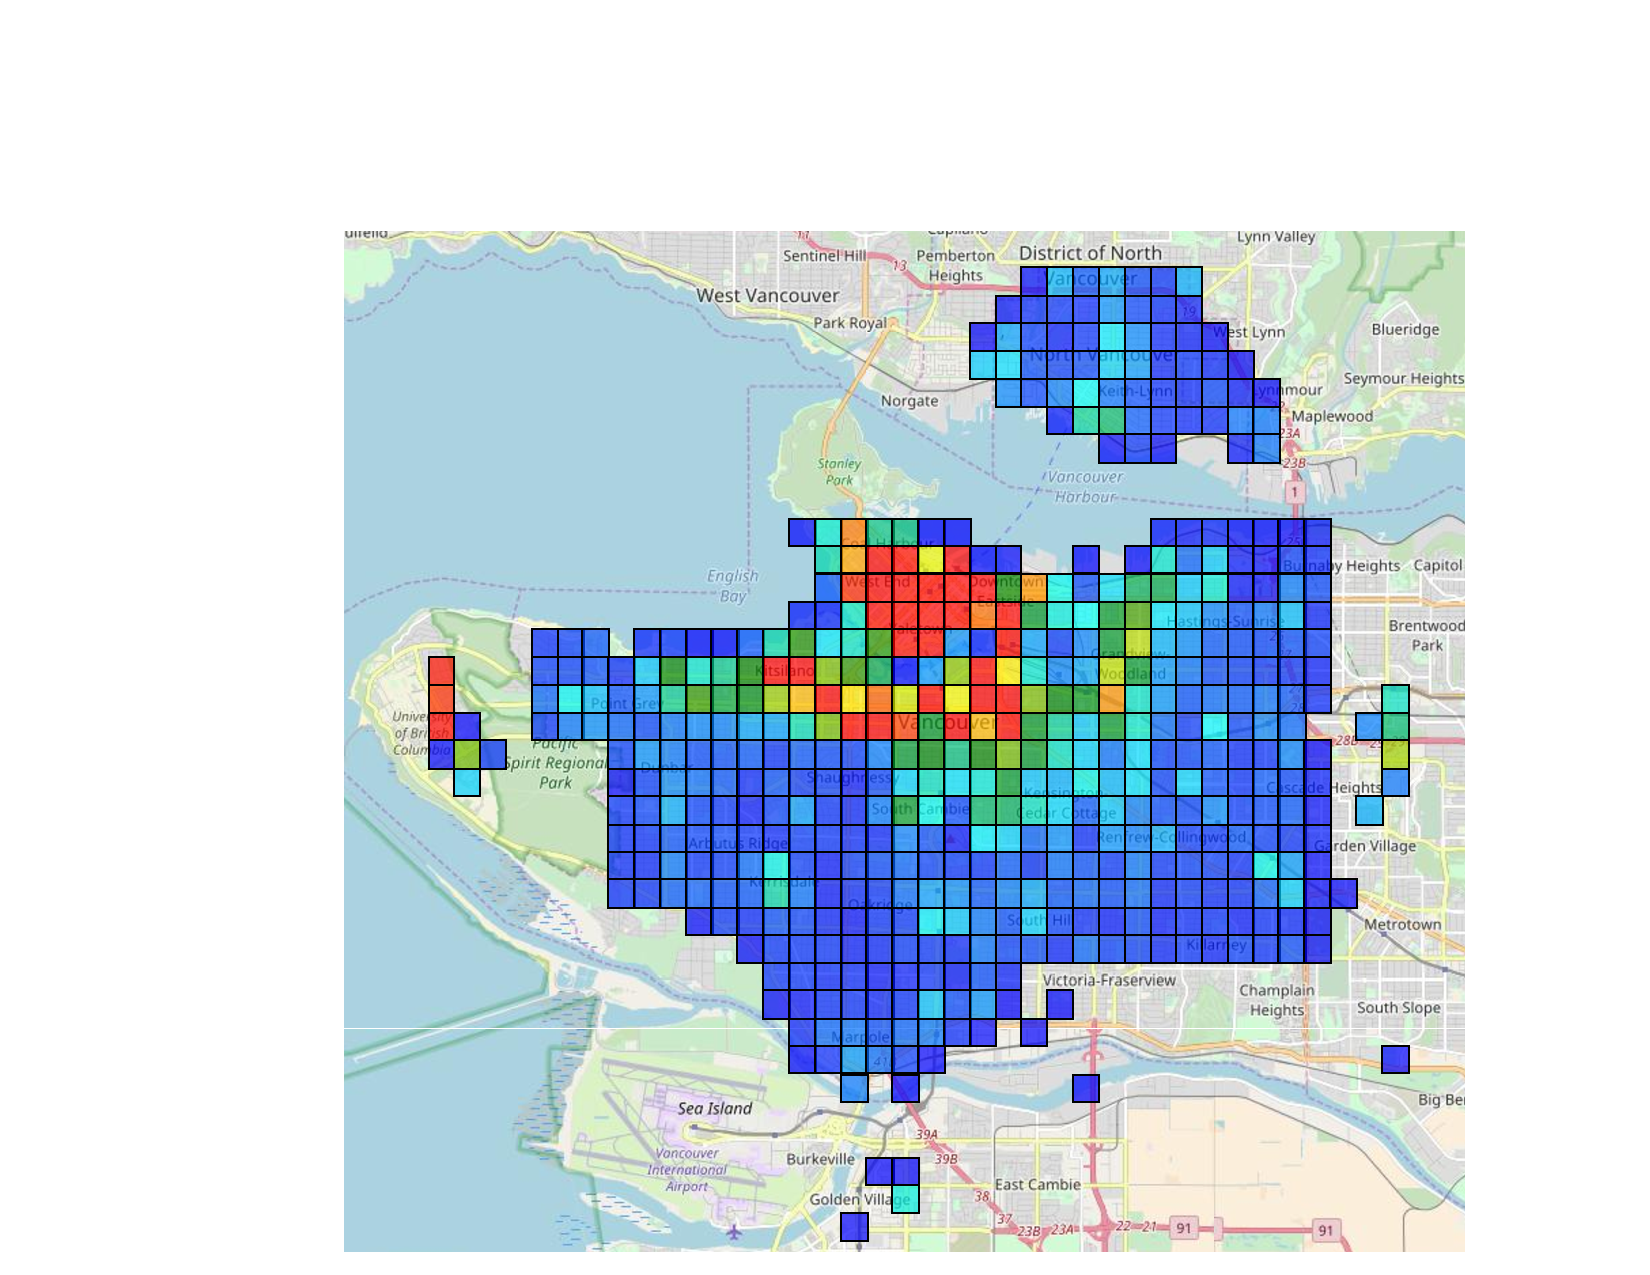
\includegraphics[width=0.30\columnwidth]{figures/VancouverMaxParking.pdf}}\label{fig:5_4_np_vancouver}}
	\quad
	\subfloat[\centering Berlin]{{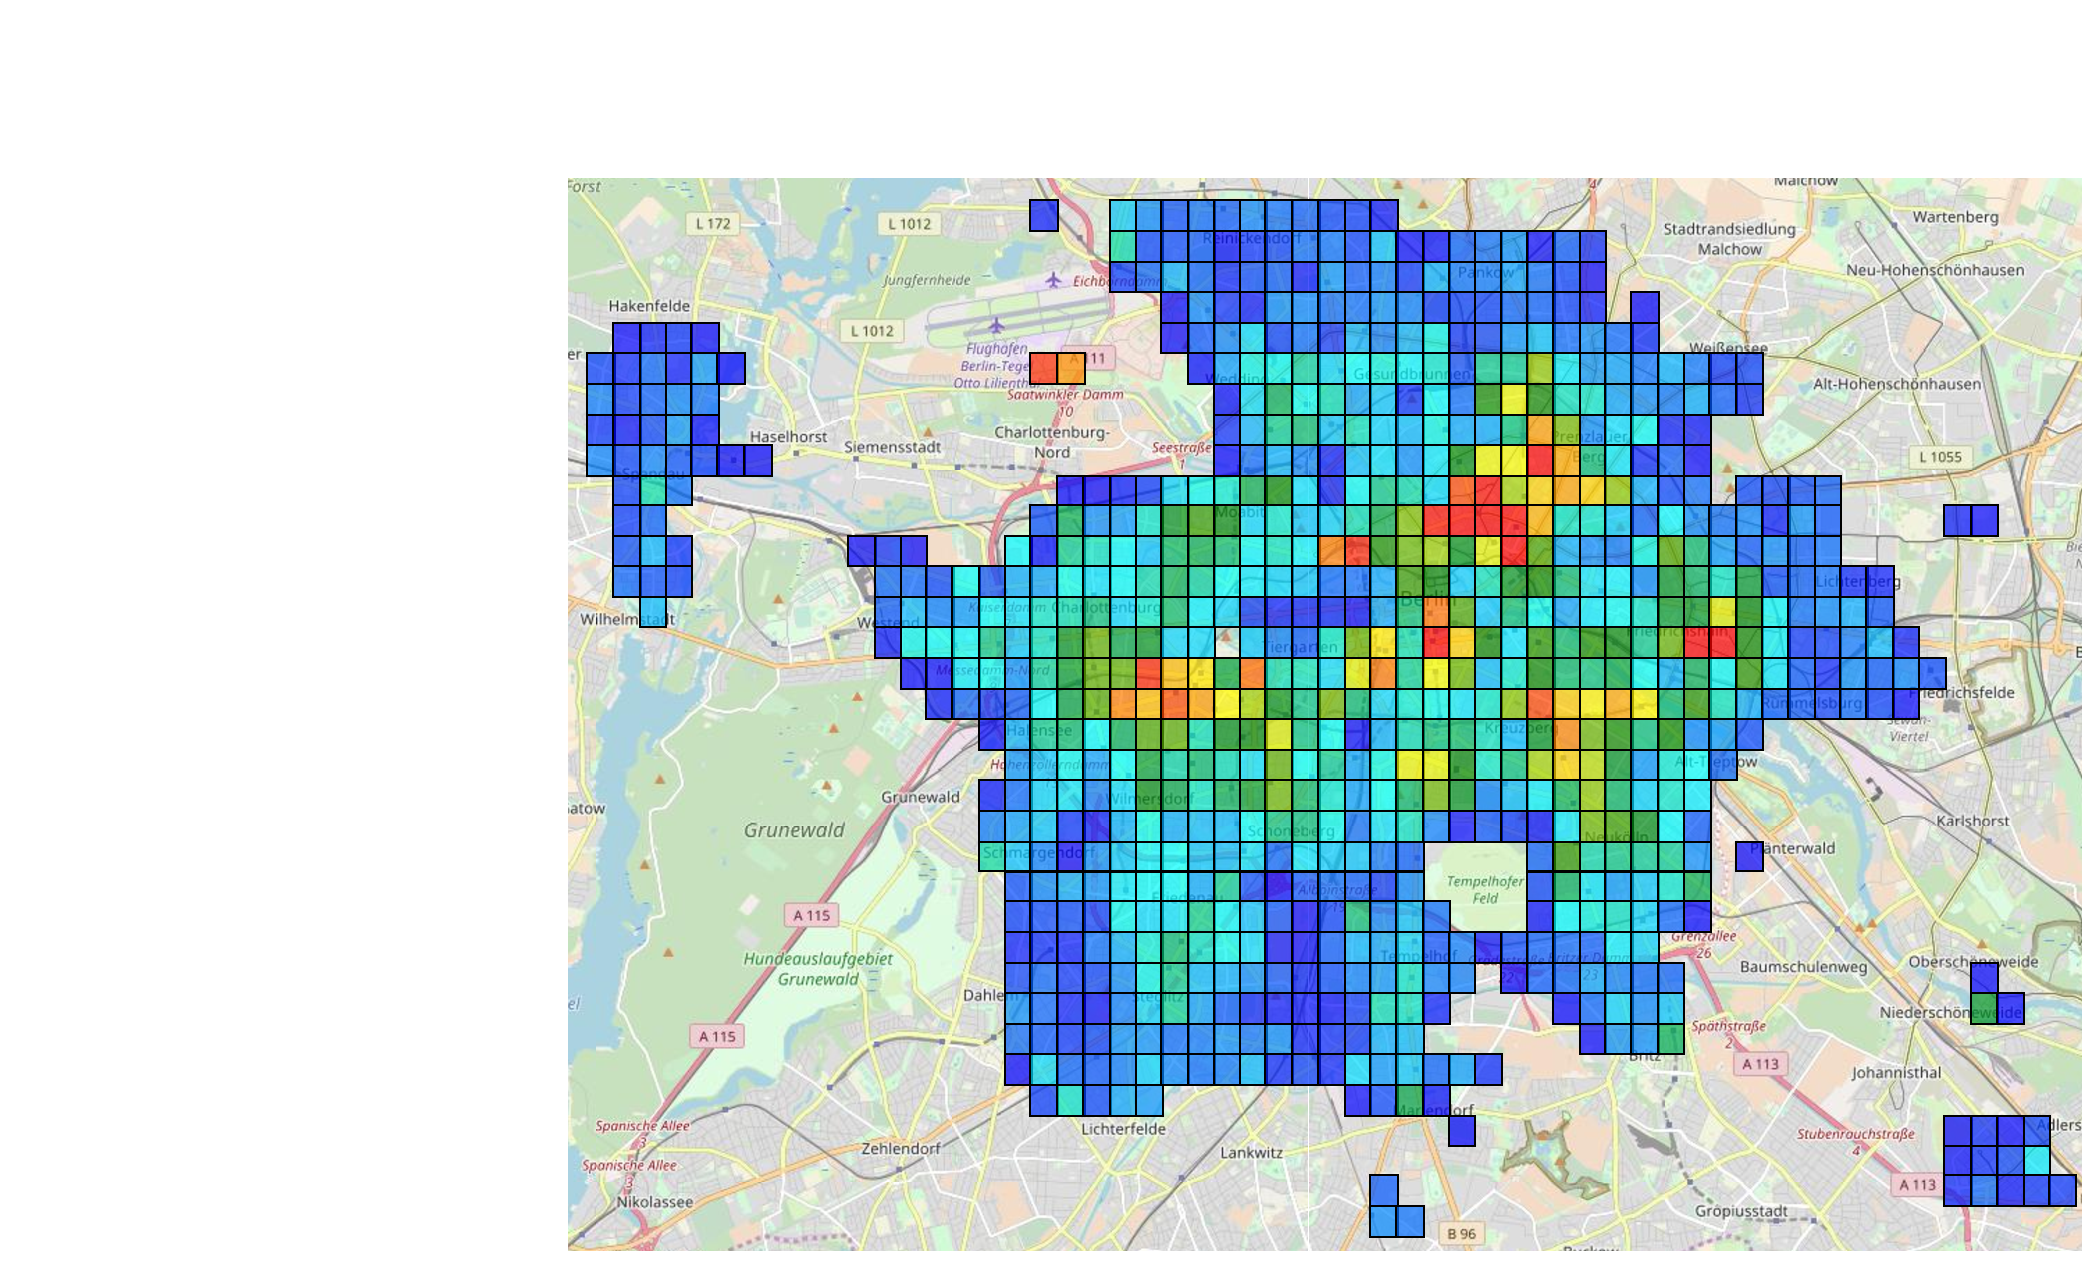
\includegraphics[width=0.4\columnwidth]{figures/BerlinoMaxParking.pdf}}\label{fig:5_4_np_berlin}}%
	\caption{Distribution of number of parking in Turin, Vancouver and Berlin}
	\label{fig:5_4_heatmap_numparking}
\end{figure}

Figure \ref{fig:5_4_heatmap_numparking} depicts the number of parking in each zone, for Turin (\ref{fig:5_4_np_turin}), Vancouver (\ref{fig:5_4_np_vancouver}) and Berlin (\ref{fig:5_4_np_berlin}). Reminding that more parkings means an higher zone attractiveness,
 it is possible to notice how the zones with the highest number of parking concentration zones are delimited in particular areas. For example figure \ref{fig:5_4_np_turin} shows how most frequented areas are downtown in correspondence of the two main train stations and the airport. A similar pattern can be spot in figure \ref{fig:5_4_np_vancouver}. Contrary, Berlin presents at least three actractive areas. This is mainly due to the biggest operative area and, probably, to the differentiation of business areas.

This brief catheterization shows how  different cities can have different spatial characterization and thus different charging station placements. However those characterization will be deepened in chapters \mc{captoli}.


\section{Users' Plugging Policy}
\label{sec:5_4_return_policy}
One of the most challenging points of electric FFCS is to deal with the discomfort derived by plug in operations. This operation is more time consuming with compared to the normal filling up procedure of combustion engine cars. Therefore, the providers have to deal with users' selfishness and trying to stimulate their willingness.  
In this Section, we define different policies that the electric FFCS may enforce, and different probabilistic behaviors of customers. 

\subsection{Car charging policies}
When returning the car, the customer may connect the car to a pole in a station, hence charging the car battery and possibly deviating the real destination from the desired one. I modelled the following policies:
\begin{itemize}
	\item{\it Free Floating}: the customer must connect the car to a charging pole if and only if it is available in the desired final zone $D(i)$;
	\item{\it Forced}: cars must be connected to a pole when the percentage of battery charge at the end of the rental $i$ would go below a certain threshold $\pi$, i.e., $(c(a,t_{s}(i)) - Energy(p(a,t_{s}(i)), d(i))) \cdot 100/ C\leq  \pi $. This implies the customer can be \textit{rerouted} to the closest zone to the desired one $d(i)$, if no free pole exists in the zone; %Battery consumption takes into account the additional traveled distance.
	\item{\it Hybrid}: the customers follow the forced policy; they may  also choose to connect to a charging pole available in the desired ending zone $D(i)$ with probability $w\in [0,1]$;
	%if the $c(a,t)\leq\pi$, cars must be returned to the closest recharging zone to $d(i)$.
\end{itemize}

The \textit{Free Floating} policy never obliges the customer to bring the car far from the desired ending location, even in case battery is close to exhaustion. It used as benchmark, in order to understand until when the users might rent car without any restriction/
\textit{Forced} mandates to connect cars to a charge station only when energy runs low, thus trying to protect from battery exhaustion.
\textit{Hybrid} introduces the level of customers willingness to collaborate, named with $w$. $w=0$ is equivalent to the Forced policy, while $w=1$ adds to the Forced policy the Free Floating policy,  thus always connecting the car to a charging pole if available in their final position zone. The users' willingness should be $w$ should be intended as the probability that a user can collaborate with the provider, dropping the car in a charging station. The $w$ variability can by justified like provider incentive bonus like car2go free minutes after a car filling up.



\section{Key Performance Indicators and Simulation Scenario}

In this section, I describe which are the simulation outputs and the scenario with which I performed the analyses. In particular I focused the attention on minimum requirements to system sustainability and measuring of users discomfort. 

\subsection{Performance metrics and parameters}

The simulator measures metrics that are  key to assess in the quality of experience for the customers:
\begin{itemize}
	\item \emph{Infeasible trip}: measures if a trip $i$ performed by a car $a$ ends with a completely discharged battery, i.e., when $c(a,t_{e}(i))= 0$;
	\item \emph{Charge event}: indicates a trip $i$ that ends with putting in charge the car, implying the burden to drive to the pole position, and plug the car;
	\item \emph{Reroute event}: a trip $i$ where the customer is rerouted to a zone different from the  desired destination because forced to charge the car $a$, i.e., $P(a,t_{e}(i))\neq D(i)$;
	\item \emph{Walk distance}: distance between the desired final location $d(i)$ and the actual final position $p(a,t_{end}(i))$.
\end{itemize}

The number of infeasible trips are critical, and the system shall be engineered so that they never happen. Other performance metrics shall be minimized. 
In addition to the above metrics, the simulator collects statistics about car battery charge level $c(a,t)$, and fraction of time a battery stays under charge.

\subsection{Simulation scenario}

I used this simulator to study the impact on the number of zones that are equipped with charging stations $N$, and the number of poles $k$ of each charging station.

I consider in each city a fleet that has a number of cars equal to the one observed in the trace. Electric cars have the same nominal characteristics as the Smart ForTwo Electric Drive, i.e., $17.6\,kWh$ battery, for $135\,km$ of range, with a discharge curve $Energy()$ that is proportional to the travelled distance ($12.9\,kWh/100\,km$). \footnote{\url{https://www.smart.com/uk/en/index/smart-electric-drive.html}} 
Charging stations have $k=4$ low power ($2\,kW$) poles each. These are cheap to install and a good compromise between costs, power requested, and occupied road section. We model a simple linear charge profile (complete charge in 8 hours and 50 minutes in our case). At last, the initial car position, only affecting the simulation transient, is chosen randomly.

The simulator, written in Python, takes less then 5 seconds to complete a single simulation for a given city and parameter set. 
Due to the large number of simulations, we run them in parallel. Each simulation produces 100\,MB of detailed logs, that we process on a Big Data cluster of 30 nodes using PySpark.%\footnote{\url{http://spark.apache.org/docs/latest/api/python/\#}}.

\section{Conclusion}\label{key}
\label{sec:5_6_conclusion}
In this chapter I described a FFCS electric mobility simulator I developed. Starting from the data collected with the software described in chapter \ref{chap:2_dataset} I created trace of rental events, describing the system allocated users' demand. 

More in details, the simulator allocates a set of cars, characterized by battery capacity and power consumption per kilometres. Then consumes the rental trace, marking the car unavailable after a \textit{rental-start} event and updating the final battery state of charge when a \textit{rental-end} event is processed. Moreover, the simulator is in charge to place the charging station according three heuristics: random, preferring zones having a grater parking time and zones having the higher number of parkings. Finally it takes in account the different policies with which the users have to return the car.

When the trace is consumed, this simulator computes several key performance indicators measuring the proper system infrastructure allocation and users' discomfort to deal with an electric vehcile